\documentclass[a4paper, 11pt]{article}
\usepackage[margin=0.75in]{geometry}
\usepackage[english]{babel}
\usepackage[utf8]{inputenc}
\usepackage{amsmath}
\usepackage{graphicx}
\usepackage[colorinlistoftodos]{todonotes}
\usepackage{listings}
\usepackage{epstopdf}
\usepackage{import}
\usepackage[none]{hyphenat}
\usepackage{algorithmicx}
\usepackage{algorithm}% http://ctan.org/pkg/algorithms
\usepackage{algpseudocode}% http://ctan.org/pkg/algorithmicx

\usepackage{array}
\newcolumntype{L}[1]{>{\raggedright\let\newline\\\arraybackslash\hspace{0pt}}m{#1}}
\newcolumntype{C}[1]{>{\centering\let\newline\\\arraybackslash\hspace{0pt}}m{#1}}
\newcolumntype{R}[1]{>{\raggedleft\let\newline\\\arraybackslash\hspace{0pt}}m{#1}}

\lstset{basicstyle=\ttfamily,breaklines=true}

\title{Remote GDB debugging of AJIT Processor Cores}

\author{Titto Thomas, Madhav P. Desai\\ Department of Electrical Engg.\\ IIT Bombay\\Powai, Mumbai 400076}

\date{\today}

\begin{document}
\maketitle

\section{Introduction}

The AJIT processor is available in a variety of configurations, ranging from
a single core, single CPU thread setup to a multi-core setup with each core
having two CPU threads.    Each CPU thread implement either the SPARC-V8 ISA (the AJIT-32 thread), or
the SPARC-V8 ISA with custom  64-bit extensions (the AJIT-64 thread).  We describe the
debug setup for the AJIT processor.

The  GDB debugger is used as a remote client, while the role of the
server is performed either by 
\begin{itemize}
	\item A C emulator model of the multi-core multi-thread processor
	\item An AJIT debug monitor utility which in turn controls the execution
		of the AJIT processor using a serial USB-UART link.
\end{itemize}


\section{Using the debug setup with the AJIT C emulator model}

Currently, the AJIT C emulator models the following system:
\begin{itemize}
\item Up to 4 cores, with each core either having 1 or 2 threads.  
The threads can either be AJIT-64 threads, or AJIT-32 threads.
\item An interrupt controller, a timer, a serial device.
\item A coherent memory.
\end{itemize}

\subsection{Starting the emulation model}

The AJIT C emulator model is invoked as
\begin{verbatim}
ajit_C_system_model ... options ....
\end{verbatim}
The  options relevant for debugging are summarized below
\begin{verbatim}
-n <number-of-cores>     
      : specifies number-of-cores in the processor for this test.
      : default is 1, maximum is 4.
t <number-of-threads-per-core>     
      : specifies number-of-threads-per-core in the processor for this test.
      : default is 1, maximum is 2.
-u <32/64>
      :  use -u 64 to run model in 64-bit mode [default is 32]
-m <mmap-file>     
      : required, specifies memory-map of processor for this test.
-g, optional, to run the CORE in debug mode.
-p <gdb-port-number>, required with -g, to specify remote debug port.
-i <init-pc>, optional, for specifying  initial value of PC (default=0). NPC is PC+4
\end{verbatim}
For example, if we are debugging a machine with two cores, each of which has 
two AJIT-32 threads, we would use
\begin{verbatim}
ajit_C_system_model -m prog.mmap -n 2 -t -u 32\
   -g -p 8888 -p 8889 -p 8890 -p 8891 
\end{verbatim}
This will start four GDB servers  listening on ports 8888-8891.  Port 8888 is used for 
debugging (core=0, thread=0), port 8889 is used for debugging (core=0,thread=1) and
so on.

\subsection{Start the GDB clients}

Since we are debugging four threads, we will start four clients in four shells
(or in a TMUX session with four panes).  For example, for core,thread (0,0), we
start
\begin{verbatim}
sparc-linux-gdb prog.elf
\end{verbatim}
Now a GDB shell will start and you can see the messages shown in Fig. 1
\begin{figure}[H]
		\centering
		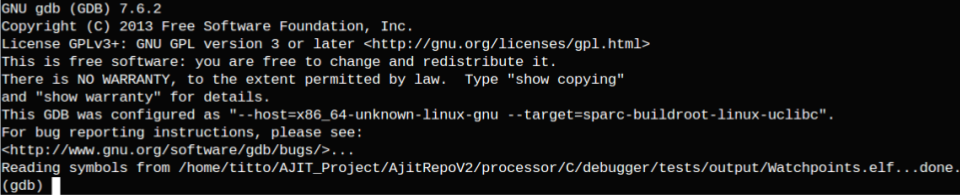
\includegraphics[width=0.8\columnwidth]{Figs/first.png}
		\caption{GDB debug session}
\end{figure}
You will need to start a shell for each thread that you are debugging.

Now in the GDB shell for core,thread (0,0), type
the same \texttt{port number}.
\begin{verbatim}
(gdb) target remote:8888
\end{verbatim}
Do the same thing in the other four shells (with the appropriate port numbers).

The gdb side will also show the following messages confirming the connection establishment. 
Since the connection has now been established, you can control and monitor the program execution on 
the AJIT thread in real time.
\begin{figure}[H]
	\centering
	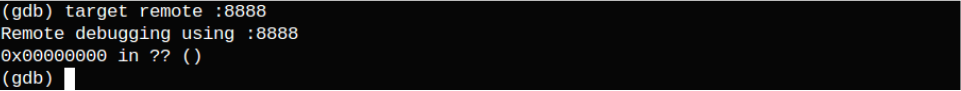
\includegraphics[width=0.8\columnwidth]{Figs/second.png}
\end{figure}

\section{Using the GDB debug setup with the ajit\_debug\_monitor\_mt utility}
TBD.

\section{Basic GDB commands for use}

\subsection*{Continue / Next}
When the execution is stopped due to some reason, you can let the processor continue with these commands.
\begin{lstlisting}[language=bash]
(gdb) continue
(gdb) c
\end{lstlisting}
Next command also lets the processor continue, but stops it after executing one more line of code.
\begin{lstlisting}[language=bash]
(gdb) next
(gdb) n
\end{lstlisting}

\subsection{Breakpoints}
Breakpoints are useful for stopping the execution on reaching specific points in the source code, and probe the processor for information. They can be set using the following commands.
\begin{lstlisting}[language=bash]
(gdb) break <function_name>
(gdb) break <line_number>
(gdb) break <filename : function_name>
(gdb) break <filename : line_number>
(gdb) break *<address>
\end{lstlisting}
Example:
\\
\begin{figure}[H]
	\centering
	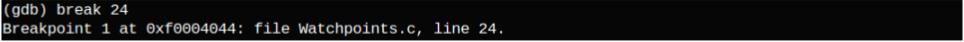
\includegraphics[width=0.8\columnwidth]{Figs/fourth.png}
\end{figure}

The AJIT thread being debugged will stop execution when a breakpoint is hit, 
and you will be notified in the corresponding GDB shell.
\begin{figure}[H]
	\centering
	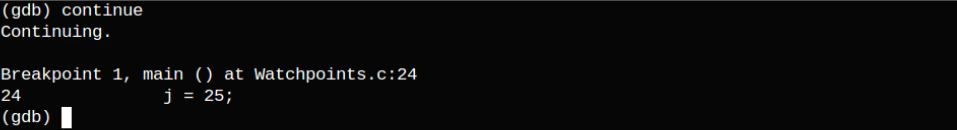
\includegraphics[width=0.8\columnwidth]{Figs/fifth.png}
\end{figure}
Breakpoints can be listed by the following command.
\begin{lstlisting}[language=bash]
(gdb) info breakpoints
\end{lstlisting}

This command can be used to delete specific breakpoints.
\begin{lstlisting}[language=bash]
(gdb) delete break <breakpoint_number>
\end{lstlisting}

\subsection{Watchpoints}
Watchpoints are useful for stopping the execution on modification of specific variables in the source code, and probe the processor for information. They can be set using the following commands.
This command can be used to delete specific breakpoints.
\begin{lstlisting}[language=bash]
(gdb) watch [-l|-location] <variable>
(gdb) break [-l|-location] <expression>
\end{lstlisting}
Ordinarily a watchpoint respects the scope of variables in expression. The \texttt{-location} argument tells gdb to instead watch the memory referred to by expression.

Example:
\begin{figure}[H]
	\centering
	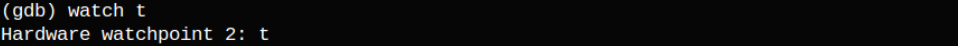
\includegraphics[width=0.8\columnwidth]{Figs/sixth.png}
\end{figure}
The AJIT thread being debugged will stop execution when a watchpoint is hit, 
and you will be notified with their values in gdb.
\begin{figure}[H]
	\centering
	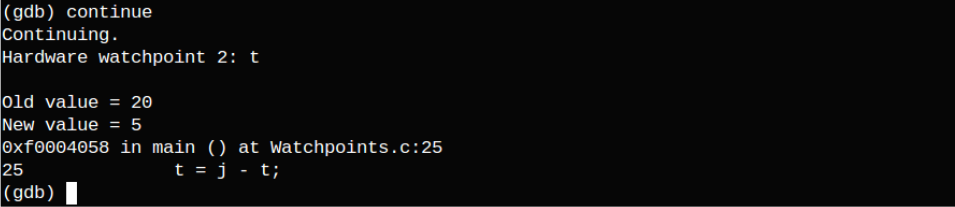
\includegraphics[width=0.8\columnwidth]{Figs/seventh.png}
\end{figure}
Watchpoints can be listed by the following command.
\begin{lstlisting}[language=bash]
(gdb) info watchpoints
\end{lstlisting}

This command can be used to delete specific watchpoints.
\begin{lstlisting}[language=bash]
(gdb) delete watch <watchpoint_number>
\end{lstlisting}

\subsection{Traps}
When the AJIT thread is executing a program, it will stop and inform the GDB
client whenever there is a trap. After a traps, you can read the \texttt{TBR} 
register to get information about the trap type etc.

Example:
\begin{figure}[H]
	\centering
	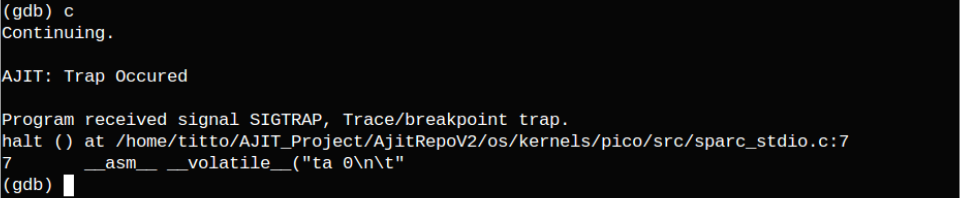
\includegraphics[width=0.8\columnwidth]{Figs/eigth.png}
\end{figure}
\subsection{Setting variables / memory / registers}
You can modify the values of variables, memory contents and register values with the set command.
\begin{lstlisting}[language=bash]
(gdb) set var <variable> = <value>
(gdb) set $ <register> = <value>
(gdb) set *(int)<memory_address> = <value>
\end{lstlisting}
Example:
\begin{figure}[H]
	\centering
	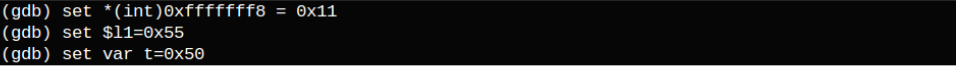
\includegraphics[width=0.8\columnwidth]{Figs/nine.png}
\end{figure}
\subsection*{Printing variables / memory / registers}
You can display the values of variables, memory contents and register values with the \texttt{print} or \texttt{p} command.
\begin{lstlisting}[language=bash]
(gdb) print var <variable>
(gdb) print $ <register>
(gdb) print *(int)<memory_address>
\end{lstlisting}
Example:
\begin{figure}[H]
	\centering
	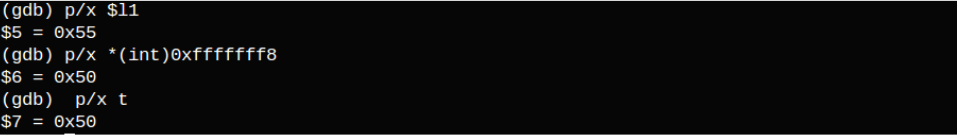
\includegraphics[width=0.8\columnwidth]{Figs/eleven.png}
\end{figure}
\subsection*{Detach}
You can stop debugging the program and let the processor continue till it finishes execution, using this command.
\begin{lstlisting}[language=bash]
(gdb) detach
\end{lstlisting}

Example:
\begin{figure}[H]
	\centering
	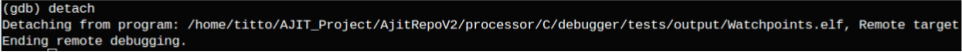
\includegraphics[width=0.8\columnwidth]{Figs/twelve.png}
\end{figure}
\subsection{Other useful commands}
You can get help on any commands using
\begin{lstlisting}[language=bash]
(gdb) h[elp]
(gdb) h[elp] <command>
\end{lstlisting}
Finish current function, loop, etc. with
\begin{lstlisting}[language=bash]
(gdb) fin[ish]
\end{lstlisting}
Show lines of code surrounding the current point
\begin{lstlisting}[language=bash]
(gdb) l[ist]
\end{lstlisting}
Delete all breakpoints
\begin{lstlisting}[language=bash]
(gdb) d[elete]
\end{lstlisting}
Add a list of gdb commands to execute each time a breakpoint is hit
\begin{lstlisting}[language=bash]
(gdb) comm[ands] <breakpoint_number>
\end{lstlisting}


\end{document}
